\section{Implementierung}\label{kapitel6}
%Code erklären, Cooler Shit, Jackson, Token, Spring Sec, srtm download?
\subsection{Webserver}
\subsubsection{Sicherheit}
Der Webserver ist mit dem Framework Spring Security abgesichert. Die Authentifizierung war dabei kein Hauptaugenmerk der Arbeit, jedoch ist sie in Grundzügen umgesetzt worden. 

So ist der Server nur allgemein abgesichert. Hat der Nutzer ein gültiges Token hat er kompletten Zugriff auf die REST-API. Das ist natürlich keine Option für ein produktives System, das seine Nutzerdaten stärker absichern muss.

Der folgende Code befindet sich in der ApplicationContext.xml und sorgt dafür, dass sämtliche Anfragen bis auf die zum Anmelden und Registrieren von Nutzern authentifiziert sein müssen.
\lstset{language=xml}
\begin{lstlisting}[frame=htrbl, caption={Ausschnit aus der Datei ApplicationContext.xml}, breaklines=true]
<security:http realm="Protected API" use-expressions="true" auto-config="false" create-session="stateless" entry-point-ref="CustomAuthenticationEntryPoint" authentication-manager-ref="authenticationManager">
        <security:custom-filter ref="authenticationTokenProcessingFilter" position="FORM_LOGIN_FILTER" />
        <security:intercept-url pattern="/login" access="permitAll"/>
        <security:intercept-url pattern="/user" method="POST" access="permitAll"/>
        <security:intercept-url pattern="/**" access="isAuthenticated()" />
    </security:http>
\end{lstlisting}
\paragraph{Anmeldung}
Um sich zu anzumelden schickt der Nutzer eine Anfrage an den Server, die eine JSON mit den Attributen ``name'' und ``password'' an den Server. Stimmen diese mit den auf einem Nutzer auf der Datenbank überein antwortet der Server mit einem Token, welches der Nutzer für drei Tage nutzen kann um die authentifizierten Bereiche der API benutzen zu können. 
\begin{figure}[htb]
\centering
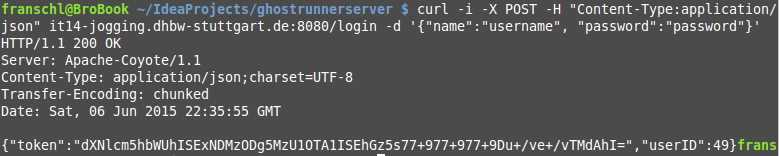
\includegraphics[width=\textwidth]{abb/curl_login}
\caption[Anmeldung]{Abbildung einer erfolgreichen Anmeldung mithilfe des Kommandozeilentools CURL}
\label{fig:Anmeldung}
\end{figure}
\paragraph{Authentifizierungstoken}
Das Authentifizierungstoken besteht, base64-dekodiert aus drei Teilen, getrennt durch jeweils drei Ausrufezeichen:
\begin{itemize}
\item Nutzername
\item Ablaufdatum des Tokens als UNIX-Zeitstempel (in Millisekunden)
\item geheimer Hash, der sich aus MD5-Hash des Nutzernamen, Salts und des Tokenablaufdatums zusammensetzt.
\end{itemize}

Dekodiert man z.B.  das erhaltene Token aus Abbildung~\ref{fig:Anmeldung} erhält man den folgenden String:
\begin{lstlisting}
username!!!1433889355905!!<einige Sonderzeichen>
\end{lstlisting}
